
\documentclass{article} % Especially this!

\usepackage[english]{babel}
\usepackage[utf8]{inputenc}
\usepackage[margin=1.5in]{geometry}
\usepackage{amsmath}
\usepackage{amsthm}
\usepackage{amsfonts}
\usepackage{amssymb}
\usepackage[usenames,dvipsnames]{xcolor}
\usepackage{graphicx}
\usepackage[siunitx]{circuitikz}
\usepackage{tikz}
\usepackage[colorinlistoftodos, color=orange!50]{todonotes}
\usepackage{hyperref}
\usepackage[numbers, square]{natbib}
\usepackage{fancybox}
\usepackage{epsfig}
\usepackage{soul}
\usepackage[framemethod=tikz]{mdframed}
\usepackage[shortlabels]{enumitem}
\usepackage[version=4]{mhchem}
\usepackage{listings}
\usepackage{epstopdf}


\epstopdfDeclareGraphicsRule{.gif}{png}{.png}{convert gif:#1 png:\OutputFile}
\AppendGraphicsExtensions{.gif}






%%%%%%%%%%%%%%%%%%%%%%%%%%
\setlength{\marginparwidth}{3.4cm}


% NEW COUNTERS
\newcounter{points}
\setcounter{points}{100}
\newcounter{spelling}
\newcounter{english}
\newcounter{units}
\newcounter{other}
\newcounter{source}
\newcounter{concept}
\newcounter{missing}
\newcounter{math}
\newcounter{terms}
\newcounter{clarity}

% COMMANDS

\definecolor{myblue}{rgb}{0.668, 0.805, 0.929}
\newcommand{\hlb}[2][myblue]{ {\sethlcolor{#1} \hl{#2}} }

\newcommand{\clarity}[2]{\todo[color=CornflowerBlue!50]{CLARITY of WRITING(#1) #2}\addtocounter{points}{#1}
\addtocounter{clarity}{#1}}

\newcommand{\other}[2]{\todo{OTHER(#1) #2} \addtocounter{points}{#1} \addtocounter{other}{#1}}

\newcommand{\spelling}{\todo[color=CornflowerBlue!50]{SPELLING (-1)} \addtocounter{points}{-1}
\addtocounter{spelling}{-1}}
\newcommand{\units}{\todo{UNITS (-1)} \addtocounter{points}{-1}
\addtocounter{units}{-1}}

\newcommand{\english}{\todo[color=CornflowerBlue!50]{SYNTAX and GRAMMAR (-1)} \addtocounter{points}{-1}
\addtocounter{english}{-1}}

\newcommand{\source}{\todo{SOURCE(S) (-2)} \addtocounter{points}{-2}
\addtocounter{source}{-2}}
\newcommand{\concept}{\todo{CONCEPT (-2)} \addtocounter{points}{-2}
\addtocounter{concept}{-2}}

\newcommand{\missing}[2]{\todo{MISSING CONTENT (#1) #2} \addtocounter{points}{#1}
\addtocounter{missing}{#1}}

\newcommand{\maths}{\todo{MATH (-1)} \addtocounter{points}{-1}
\addtocounter{math}{-1}}
\newcommand{\terms}{\todo[color=CornflowerBlue!50]{SCIENCE TERMS (-1)} \addtocounter{points}{-1}
\addtocounter{terms}{-1}}


\newcommand{\summary}[1]{
\begin{mdframed}[nobreak=true]
\begin{minipage}{\textwidth}
\vspace{0.5cm}
\begin{center}
\Large{Grade Summary} \hrule 
\end{center} \vspace{0.5cm}
General Comments: #1

\vspace{0.5cm}
Possible Points \dotfill 100 \\
Points Lost (Science Terms) \dotfill \theterms \\
Points Lost (Syntax and Grammar) \dotfill \theenglish \\
Points Lost (Spelling) \dotfill \thespelling \\
Points Lost (Units) \dotfill \theunits \\
Points Lost (Math) \dotfill \themath \\
Points Lost (Sources) \dotfill \thesource \\
Points Lost (Concept) \dotfill \theconcept \\
Points Lost (Missing Content) \dotfill \themissing \\
Points Lost (Clarity of Writing) \dotfill \theclarity \\
Other \dotfill \theother \\[0.5cm]
\begin{center}
\large{\textbf{Grade:} \fbox{\thepoints}}
\end{center}
\end{minipage}
\end{mdframed}}

%#########################################################

%To use symbols for footnotes
\renewcommand*{\thefootnote}{\fnsymbol{footnote}}
%To change footnotes back to numbers uncomment the following line
%\renewcommand*{\thefootnote}{\arabic{footnote}}

% Enable this command to adjust line spacing for inline math equations.
% \everymath{\displaystyle}


%title
\title{
\normalfont \normalsize 
\textsc{Indian Institute of Technology Bombay \\ 
CS684 Autumn Semester 2016} \\
[10pt] 
\rule{\linewidth}{0.5pt} \\[6pt] 
\huge Temperature Sensor(LM35) and LCD\\
\rule{\linewidth}{2pt}  \\[10pt]
}
\author{E.R.T.S. Lab}
\date{\normalsize \today}

\begin{document}

\maketitle
\noindent

%lab Objective
\section{Lab Objective}
% Yada Yada Yada
In this lab, you will interface a 16x2 LCD with the TIVA board and LM35 temperature sensor.

\section{Pre-requisite}
\begin{enumerate}
\item 
Lab 4 : ADC and UART
\item You may want to read about interfacing working of 16x2 lcd and interfacing it in 4 bit mode.

\end{enumerate}


%%% Problem Statement
\section{Problem Statement}

% Materials go here
%%%%%%%%%%%%%%%%%%%%%%%
% FOR A NUMBERED LIST
% \begin{enumerate}
% \item Your_Item
% \end{enumerate}
%%%%%%%%%%%%%%%%%%%%%%%
% FOR A BULLETED LIST
% \begin{itemize}
% \item Your_Item
% \end{itemize}
%%%%%%%%%%%%%%%%%%%%%%%
\begin{enumerate}
\item 
Interface a 16x2 LCD in 4 bit mode with the board. There is an onboard temperature sensor, display the temperature sensed by this sensor on the LCD; use the internal ADC to convert analog readings to digital ones.
\newline
Follow the display format as shown in the figure 1 below:
\begin{figure}
\centering
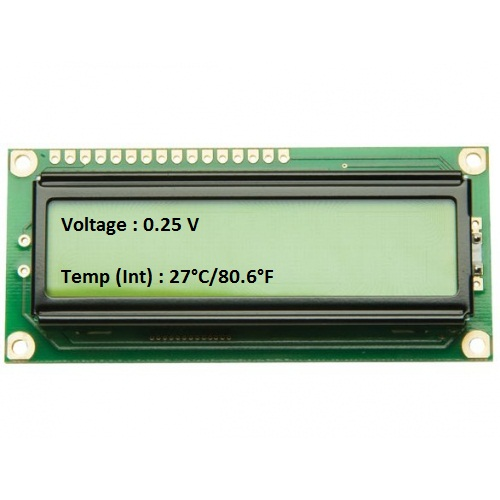
\includegraphics[scale=0.4]{16-2-lcd-backlight-green-2-500x500.jpg}
\caption{LCD Display Format}
\end{figure}
\item
Next, interface an external LM35 temperature sensor with the board and display the temperature on the LCD. Use the switch "sw1" to switch between internal and external temperature readings. The display should show external sensor readings by default and switch to internal when"sw1" is pressed once, on the next press the display should return to default (show external temperature readings). Figure 2 below will clear things out. 
\end{enumerate}
\begin{figure}
\centering
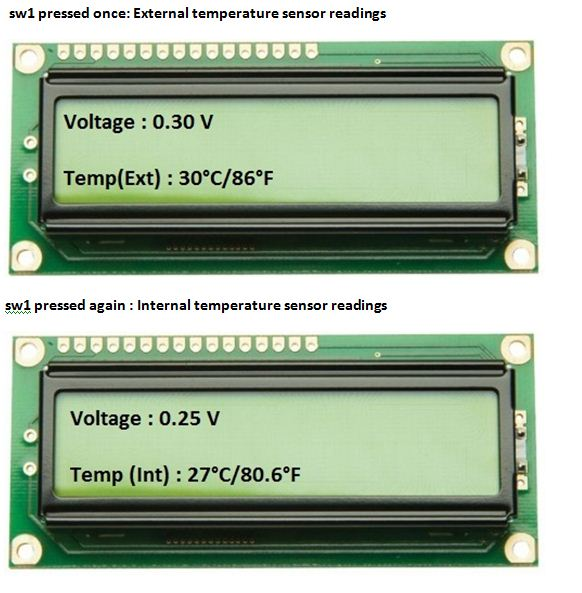
\includegraphics[scale=0.5]{flow.JPG}
\caption{Alternating sensor display values}
\end{figure}




%Relevant Theory
\newpage
\section {Relevant Theory}
%%%%%%%%%%%%%%%%%%%%%%%
% FOR A NUMBERED LIST
% \begin{enumerate}
% \item Your_Item
% \end{enumerate}
%%%%%%%%%%%%%%%%%%%%%%%

This lab will use LM35 temperature sensor, you can refer to its datasheet from the following link:\href{http://www.ti.com/product/LM35/datasheet}{\textbf{Datasheet}}.
\\
\\
You have to interface LCD in 4 bit mode rather than 8 bits. Read up about LCD working and the basic LCD commands to be used for initialization.
\newline
\\
\\
The problem statement requires you display decimal values upto two places on the LCD. You can shift the values to the left by appropriate places and then use the ascii value of "." to display decimal values.  
\\
\\
Please follow the timings given in the LCD data sheet during initialization. 
\\
Make the code modular with header file etc so that you can seamlessly use LCD for other projects as well.
%%%Procedure
%%%%%%%%%%%%%%%%%%%%%%%%%%%%%%
\section {Procedure}
%%%%%%%%%%%%%%%%%%%%%%%%%%%%%%
% TO IMPORT AN IMAGE
% UPLOAD IT FIRST (HIT THE PROJECT BUTTON TO SHOW FILES)
% KEEP THE NAME SHORT WITH NO SPACES!
% TYPE THE FOLLOWING WITH THE NAME OF YOUR FILE
% DON'T INCLUDE THE FILE EXTENSION
% \includegraphics[width=\textwidth]{name_of_file}
% \textwidth makes the picture the width of the paragraphs
%%%%%%%%%%%%%%%%%%%%%%%%%%%%%%
% TO CREATE A FIGURE WITH A NUMBER AND CAPTION
% \begin{figure}
% \includegraphics[width=\textwidth]{image}
% \caption{Your Caption Goes Here}
% \label{your_label}
% \end{figure}
% REFER TO YOUR FIGURE LATER WITH
% \ref{your_label}
% LABELS NEED TO BE ONE WORD
%%%%%%%%%%%%%%%%%%%%%%%%%%%%%
\begin{enumerate}
\item For LCD in 4 bit mode :\\
First initialize lcd in 4 bit mode\\
Give commands for clear screen,display on and cursor location\\
Command mode:\\
In command mode rs=0 and rw=0\\
Send higher 4 bit\\ 
After sending data to the port;give a enable pulse \\
Send lower 4 bit\\ 
After sending data to the port;give a enable pulse \\
Give delay of microsecond at end\\
Write mode:\\
In write mode rs=1 and rw=0\\
Send higher 4 bit\\ 
After sending data to the port;give a enable pulse \\
Send lower 4 bit\\ 
After sending data to the port;give a enable pulse \\
Give delay of microsecond at end\\
\item For external tenprature conversion:\\
Configure adc1 chip\\
set ch1 to get analog data\\
enable adc1 \\
wait untill interrupt has occured\\
store the data in the variable and convert it into celsius by dividing it with 12.41\\
convert the stored data into character and store it in array\\
send the character array to lcd screen\\
\item For internal temprature\\
Configure adc0 chip\\
set the temprature given on chip\\
enable adc0\\
wait untill interrupt has occured\\
store the data in variable and convert data into celcius\\
convert the stored data into character and store it in array\\
send the character array to lcd screen\\






\end{enumerate}


%%% Demo and Submissions
\section {Demo and Submissions}
%%%%%%%%%%%%%%%%%%%%%%%%%%%%%%%%%%%%%%%%%%%%%%%%
You have to shoot two individual videos demonstrating the output of the problem statement.
Your codes for each of the problem statement has to be uploaded in Github repository.








%\subsection{Definitions}
% Include your sources!
%%%%%%%%%%%%%%%%%%%%%%%
% LIST OF DEFINITIONS
% \begin{description}
% \item [WORD] {Definition}
% \end{description}
%%%%%%%%%%%%%%%%%%%%%%%






%\subsection{Results}
% State your main discovery based on the experimental data.






%\subsection{Questions}
% Write full question and format answers in ITALIC
% CTRL + I for ITALIC













% USE NOCITE TO ADD SOURCES TO THE BIBLIOGRAPHY WITHOUT SPECIFICALLY CITING THEM IN THE DOCUMENT

%\nocite{ref_num}


%%%%%%%%%%%%%%%%%%%%%%%%%%%%%%%%%%%%%%%%%%%%%%%%%%%%%%

			% BIBLIOGRAPHY: %

% Make sure your class *.bib file is uploaded to this project by clicking the project button > add files. Change 'sample' below to the name of your file without the .bib extension.
%%%%%%%%%%%%%%%%%%%%%%%%%%%%%%%%%%%%%%%%%%%%%%%%%%

%\bibliographystyle{plainnat}
%\bibliography{sample}

% UNCOMMENT THE TWO LINES ABOVE TO ENABLE BIBLIOGRAPHY

%%%%%%%%%%%%%%%%%%%%%%%%%%%%%%%%%%%%%%%%%%%%%%%%%%


\end{document} % NOTHING AFTER THIS LINE IS PART OF THE DOCUMENT
